%!TEX root = ../thesis.tex

\cleardoublepage
\chapter{Evaluation}
\label{cha:evaluation}

This chapter looks at the results achieved and considers their origins as well as their implications going forwards. In section \ref{sec:analysis} the results are presented and analysed. Then  section \ref{sec:_pot_improvements} considers what could be improved or done differently . Finally section \ref{sec:implications} looks forwards and asks what implications this could have and what the next steps would be.


\section{Testing the Agents}
\label{sec:testing}

In order to evaluate the performance of these agents they were tested on a 32-core, 125GB RAM machine against 5 different workflows. Each workflow is run 10 times without any reinforcement learning agents active. This was done to have something to compare the results to later but also so that there was historical data about the average time each of the tasks take since the reinforcement learning agents need this information. After that the agents are tested. The gradient bandits are run 50 times for each workflow and the Q-learning agents 100 times.

The input data used for the workflows is based on custom combinations of different input files provided by the workflow's maintainers- there are the full example datasets and the short example datasets. The combinations are designed to strike a balance between having large input data and realistic task configurations but also being short enough that it is feasible to run the workflows hundreds of times. For reference, the full datasets will often take 6 hours or more to run once whereas the short examples never take more than 5 minutes. 

The nextflow source code inherently keeps track of the total number of resources available and the resources already assigned to tasks and it will not schedule more resources than the system has. The tasks are all run inside of docker containers with exactly number of CPUs and memory requested by the task. 

For the final comparison in the evaluation chapter the 10 runs without the agents were compared to the last 10 runs with each of the agents.



%%=========================================
\section{Analysis of Results}
\label{sec:analysis}

\subsection{Performance Comparison}
\label{sub:comp_perf}

\begin{figure}
    \centering
        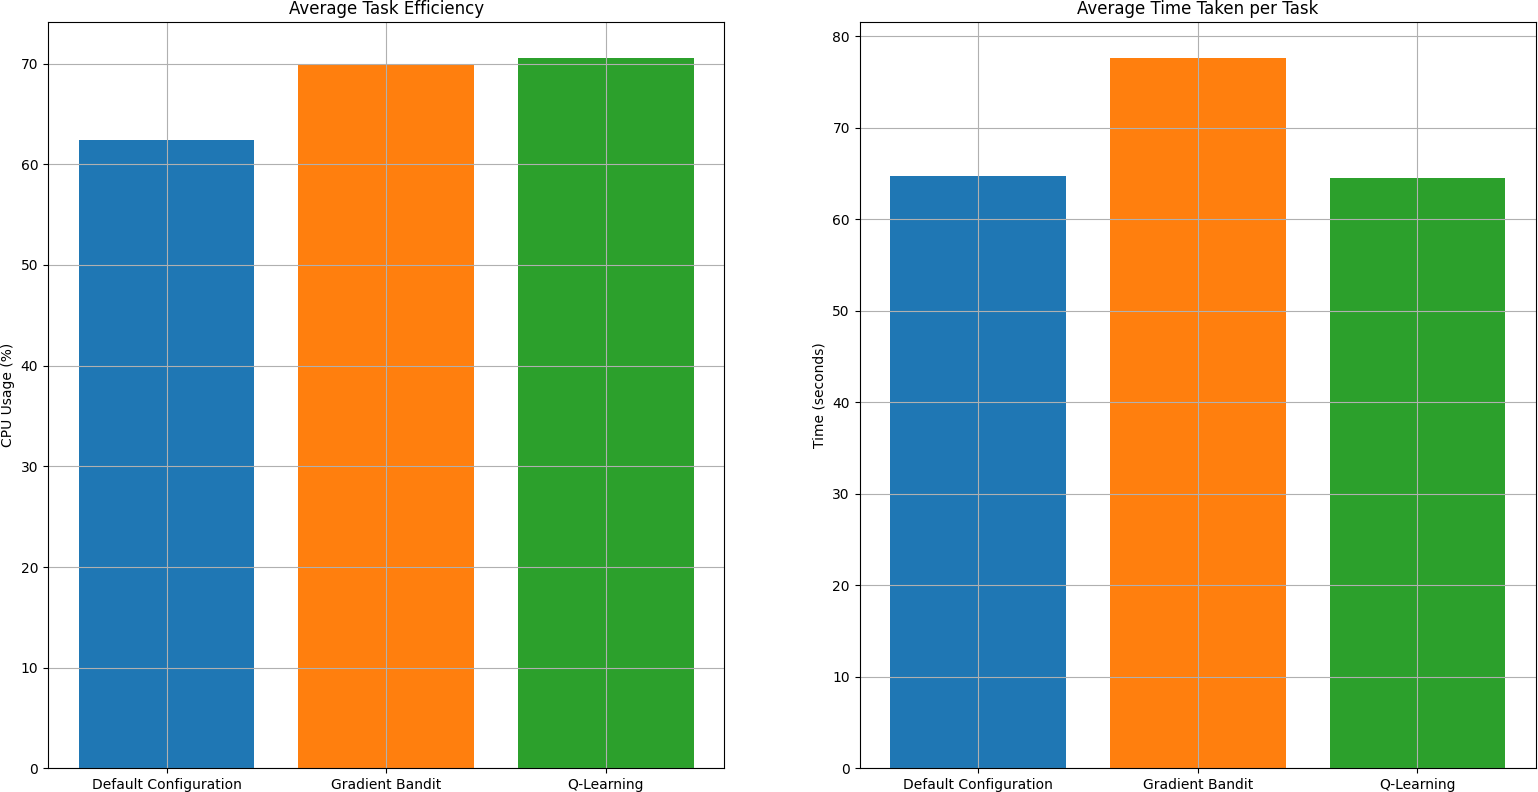
\includegraphics[width=\textwidth]{fig/cropped_per_task_results.png}
        \caption{Comparison of Average Task Efficiencies and Runtimes}
        \label{fig:task_results}
\end{figure}

\begin{figure}
    \centering
        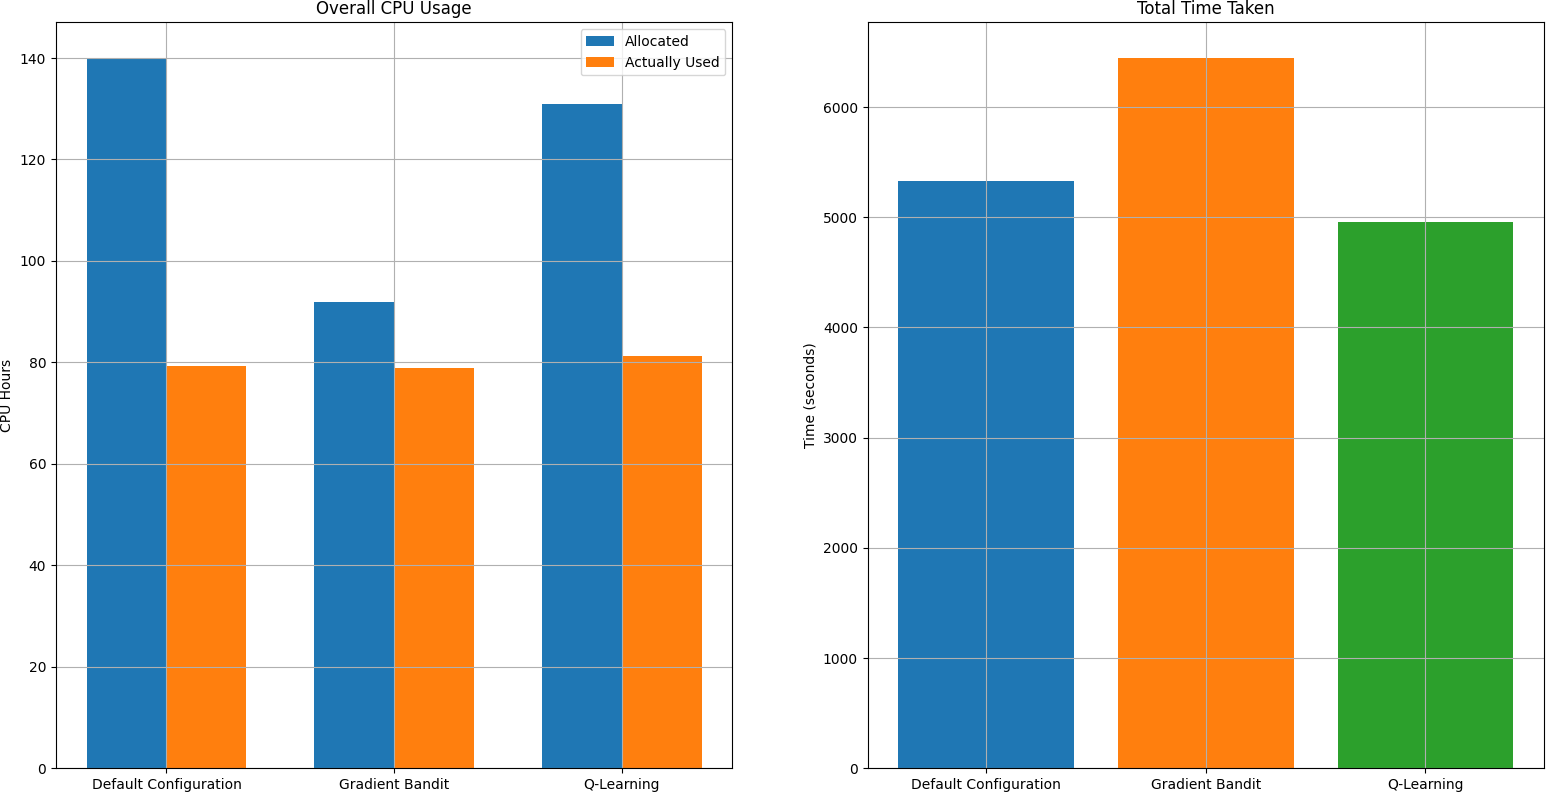
\includegraphics[width=\textwidth]{fig/cropped_wf_results.png}
        \caption{Average Performance of the Workflows}
        \label{fig:wf_results}
\end{figure}

\begin{figure}
    \centering
        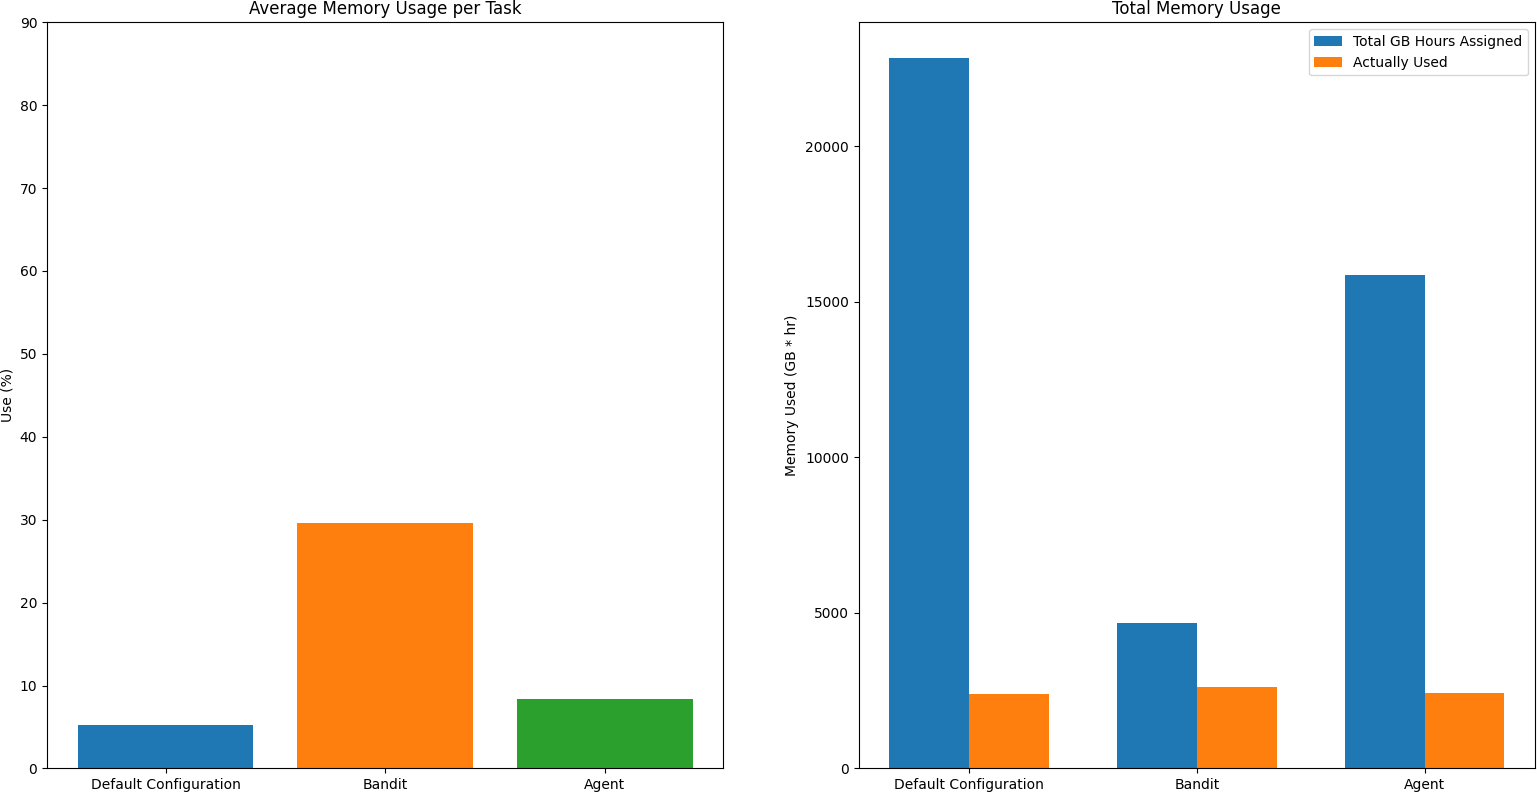
\includegraphics[width=\textwidth]{fig/cropped_memory_usage_final.png}
        \caption{Memory Usage}
        \label{fig:mem_use}
\end{figure}

Here the performance of the gradient bandit and the q-learning approach over their last 10 instances will be compared with the performance of 10 instances of the same sets of workflows when run with their default configuration.

The figures \ref{fig:task_results} and \ref{fig:wf_results} show the performance of the different approaches and compare them to the default configuration. The left graph in the first figure looks at the CPU usage on a task by task basis whereas the left graph in the second figure is displays the total amount of CPU hours requested by by all of the tasks across all of the workflows and the amount of CPU hours that were actually used. Similarly, the right graph in figure \ref{fig:task_results} is the average time the tasks took whereas the right graph of figure \ref{fig:wf_results} shows the total time it took for all of the workflows to complete. Finally in \ref{fig:mem_use}, the memory usage is shown. The unit measured is the gigabyte hour and the graphic displays the total amount of gigabyte hours allocated across all of the runs as well as the actual amount of gigabyte hours used (based on the task’s peak RSS and execution time). The gradient bandit is not shown in this figure because it did not alter memory configurations.

From these graphics it is clear to see that both of the reinforcement learning approaches managed to improve the CPU efficiency of the individual tasks as well as allocating less CPU Hours across the entire workflow. In the case of the gradient bandit it was particularly effective at keeping the overall CPU hours assigned to an absolute minimum however the actual efficiency of this approach on a task by task level was not significantly better than the q-learning agent. However it seems that the gradient bandit's efficiency came at the cost of speed and it performed worse in this aspect. The q-learning approach was less efficient overall than the gradient bandit but it had the highest average efficiency per task and took the least time. Indeed the q-learning approach was both more efficient and faster than the default configurations and it used a great deal less memory. Memory is of the course last metric by which the q-learning agent could be judged and in the end it proved to be significantly better with regards to this resource.

\subsection{Explanation}
\label{sub:explanation}

One fact which may immediately jump out is that while the q-learning agent is slightly more efficient on a task by task basis than the gradient bandit, it is significantly less efficient from the perspective of CPU hours. This must mean that the gradient bandit performs better for longer tasks (and thus uses less CPU hours overall) but for most tasks the bandit and the agent behave similarly. This might also explain why the q-learning agent is faster- if it were choosing to assign more resources to the longest tasks it would be quicker but less efficient overall. Another possible explanation for the improved performance of the q-learning agent is that because it also reduces the overall memory usage it may be able to achieve a higher throughput. Recall that nextflow has a built in scheduler which never assigns more resources than the system has available. If there had been high memory tasks then these tasks may have been preventing other tasks from running and therefore by lowering the overall memory usage (and the overall number of CPU hours used) the q-learning agent may have increased the number of tasks running in parallel and thus sped up the workflow. 

\subsection{Summary of Results}
\label{sub:summary}

In conclusion both of the reinforcement learning approaches were able to intelligently size the tasks which comprised the workflows and in the end the overall number of CPU hours required was less and indeed the percentage of those CPU hours which were wasted was reduced. In addition to this the q-learning agent was also able to significantly reduce the memory usage. The gradient bandit took slightly longer on average but was much more efficient for that whilst the q-learning agent struck a better balance between resource efficiency and increased performance and was ultimately able to outperform the default configurations with regards to both efficiency and time.

While it could be argued that the q-learning agent is therefore the “better” option it is hard to say exactly what the right approach is because it also depends on the desires of the user. Many scientists may be prepared to accept slightly longer run times if the “niceness” of the workflows is increased and they are able to free up resources for others to use at the same time or reduce their own costs (if they are paying for CPU hours). Indeed from a financial perspective the gradient bandit wastes significantly less CPU hours than the extra time it takes to complete. However in a situation where the user is paying for the entire system it would make more sense from a financial perspective to use the q-learning agent approach since it reduces the amount of time for which the system needs to be up.

%%=========================================
\section{Potential Improvements}
\label{sec:pot_improvement}

Immediately the most obvious area in which these two approaches could be improved upon would be to incorporate read and write calls into the reward function. When a thread reads or writes characters from or to a device it must perform a system call and wait for it to complete and during this time the thread cannot use the CPU. If a program has a high degree of parallel operations but also has to read and write lots of characters then it would probably have lower CPU usage (because of the many system calls) but simultaneously would benefit from being assigned more CPUs (because it is parallelizable). However because of the nature of the bandit and the agent’s reward functions it is unlikely that this task would be assigned more resources simply because the number of read and write calls are not considered.

One aspect which weakened the gradient bandit is the disconnected nature of its model of the available actions. It cannot understand that actions which assign more resources are all quite similar. From the perspective of the gradient bandit all of its actions have the same probability of success and it can’t tell when actions are very similar. As an example the decisions to assign 5 CPUs or 6 CPUs to a task which has been exhibiting low CPU usage are considered two completely independent decisions even though they both fundamentally assign more resources and indeed if the assignment of 5 CPUs is not particularly successful then 6 CPUs can be expected to be even worse. The q-learning agent, on the other hand, while it cannot actually tell if certain actions are similar, can only increase or decrease the resources one step at a time and thus is unable to land in states of extreme excess or insufficiency. Returning to the previous example - if assigning 5 CPUs was unsuccessful then the agent is unlikely to return to that state and thus will not even be able to consider the question of whether or not to assign 6 CPUs. 

A different issue which was relevant to both approaches was the length of time needed to train the agents. The gradient bandit required 40 runs and the q-learning agent took 90 runs before they were tested and for large scale workflows this is a considerable amount of time to spend. Of course the agents are able to learn on the go and the performance during the training time is not so much worse as to make the workflows unusable during that time, so it really depends on the user and how often they use a given workflow. 

Finally by training the agents using the same inputs there is a danger of overfitting the agents’ resource assignments. This may be less of a danger for the CPU assignments, because the character of a task’s CPU usage is less dependent on the input and mores so on the task itself- but repeatedly using the same inputs for an agent which sizes tasks for memory does present a real danger of overfitting. This is because the memory footprint of a task is much more dependent on the input to the task and could indeed mean that the agents might learn a less performant memory allocation.

%%=========================================
\section{Implications and Further Areas of Research}
\label{sec:implications}

The obvious implications of these findings are that much like some of the scheduling problems mentioned in chapter 2, this is also an area in which reinforcement learning has interesting potential. Additionally it has also gone to show that the resource configurations in scientific workflows have room for improvement and are another area which could be researched further. Nextflow and other scientific workflow managers represent a new class of actor in the interactions between user, application and execution platform. These workflow managers do no manage the execution platform and they do not create the workflows which are executed. They are a kind of middle man and thus present a unique opportunity. Normally the interactions in such an environment are between the user and the execution platform. The user has control over both the requests for resources and the tasks while the execution platform has control over the execution at a granular level. However in the context of a scientific workflow using a workflow manager, the manager sits in between the user and the execution platform and has no control over the tasks that must be executed nor over the execution itself (this is configured by the user and managed by the execution platform). It is only capable of scheduling and sizing the tasks. This position requires a slightly different approach to common problems such as scheduling and resource assignment but it also presents an interesting avenue for research and novel approaches to these familiar problems.

Following along this train of thought, an interesting area for further research would be incorporating a machine learning approach into the scientific workflows internal scheduler. Whilst the reinforcement learning agents used for each individual task had no knowledge of the other tasks and dependencies in the workflow a scheduler would be able to have the full picture of all workflows digraph and could perhaps improve performance to a greater degree. 

The last area of research which could prove interesting would go in the opposite direction and would be to incorporate simpler, unintelligent approaches into the sizing of tasks. For example the memory assigned to a task could be picked based on the average of the peak RSS of the task during its previous runs. Likewise, the number of CPUs assigned could be based on a linear regression which tests various different CPU assignments and then uses a line of best fit to model a function of CPUs and rewards and then attempts to pick the minimizing or maximizing parameter.

Lastly, improvement on the approach presented here using either a different reward function, a custom policy combined an on-policy reinforcement learning algorithm such as TD-learning, deep q-learning which could use a neural network to model the reward function and thus reduce exploration time, or an approach which uses fractional CPUs to containers (since containers can be assigned e.g. 1.5 CPUs) for fine-grained resource assignment, all could prove to be very interesting for further research.


























%TODO: approach which schedules or considers the whole workflow, AOI-> “un” intelligent approaches (average or regression). Test the performance when training workflows with small data and running the full wf’s

